%!TEX root = proj_report_outline.tex
\chapter{Background}

This chapter aims to provide background on the innovation ecosystem and contextualise where in this landscape PitchHub fits in. First, this chapter introduces the concept of an innovation community, and explores the roles that are present within this community. Second, this chapter discusses innovation online and what security issues are raised in this environment. Third, this chapter describes the current collaborative platforms being used in the innovation space and establishes where each stands within the role taxonomy. Fourth, this chapter concludes by discussing the importance of database security and provides background on Shamir's Secret Sharing scheme.

\section{Innovation Community}
In this world of constant communication the creation of ideas is an activity no longer isolated to inventors or researchers. It has evolved into what can instead be seen as a collaborative effort from a diverse community of actors. Von Hippel defined innovation communities as ``nodes consisting of individuals or firms interconnected by information transfer links which may involve face-to-face, electronic, or other communication'' \cite{von2005democratizing}. The world of innovation today now includes actors from increasingly disparate domains who are able to contribute their unique capabilities to the innovation process \cite{che2003optimal}. The influx of unique skills being mixed into the innovation commuity has resulted in more unique opportunities for innovation being made possible. Therefore to encourage innovation is to also encourage the innovation community as well.

\section{Common Roles in Innovation}\label{commonRolesInInnovation}

The process of driving an idea from its conceptualisation to its realisation commonly requires a variety of actors. These actors as a team bring together the knowledge, skills and resources required to action the idea's fulfillment \cite{engelberger1982robotics}. For example, the Apple ][ came to being with Steve Wozniak providing the technical knowledge and skills, Steve Jobs providing the project goals and marketing drive, and Mike Markulla providing the resources to finance the operation \cite{livingston2007founders}. This is a recurring pattern, where subgroups of a team producing an innovative product or service have different responsibilities in regards to the end product or service's realisation. To formalise these common responsibilities Callaghan Innovation has identified four distinct roles that are embodied within the innovation process:

\begin{itemize}
	\item Challenger
	\item Enabler
	\item Solver
	\item Facilitator
\end{itemize}

Challengers provide the idea or problem to be solved in order to realise a business opporunity. Enablers provide the resources required to action the innovation, this may be in terms of man-power, assets or financing. Solvers provide the answer to the idea or problem presented by the Challenger(s). Facilitators provide the connections to drive the innovation's execution, this may be in terms of connecting the idea to other people or helping the idea gain reputation. In most cases these roles are too large for one person to embody them all. To continue with the Apple ][ example, we may catergorise Steve Jobs as a Challenger, asking why computers can't serve the consumer market, Steve Wozniak can be seen as an Enabler and Solver, as he both designed the Apple ][ and built them, and Mike Markulla, can be regarded as an Enabler and Facilitator, as he financed the production and also lent his reputation to the product. By recognising these roles and the interplay required between them to action an innovative idea, we can then also recognise that platforms which seek to encourage innovation must also provide functionality for the collaboration/networking between actors fulfilling these roles.

\section{Innovation Online}
One of the key technologies in the modern world is the internet. With the internet, communication and knowledge sharing has never been more accessible or easy. Naturally, the inherenet networking that is now an integral part of the innovation process has been enhanced by the internet with the reach it affords. This increased reach has allowed innovation communities to capitalise on the larger source of innovative potential and knowledge \cite{hautz2010establish}.

\section{Security, Privacy, and Trust in Online Communities}

The nature of bringing the innovation process online consequently involves bringing what could be commercially sensitive information online also. In recent times there has been a growing trend of online security attacks where user data has been compromised. Given this reality, there is a large amount of trust involved where users are relying on the platforms they are inputting their sensitive data into to take precautions to keep this data safe. Research within the domain of Economics has shown the importance of trust in a business context: ``without trust, risk is paralyzing; transactions simply do not take place'' \cite{boyd2002community}, this notion is similarly applicable in the online innovation space where users are transacting in intellectual property and skills rather than money. This trust enables users to operate in an unsafe environment. It can be regarded as unsafe as users little power over how their data is stored and once it is stored they have no control over who can view. It is therefore important for platforms to make good on this trust, first by, implementing safeguards against security threats and second by, providing functionality that gives users control over the visibility of their data.
\par
Unfortunately, the security of online communities does not solely depend on their technical security. As explored by \citeauthor{johnson2012facebook} in their work regarding Facebook and privacy \cite{johnson2012facebook} social networks also face the problem of managing insider threat. Insider threat is where users innappropriately share content with members on the network. This problem is raised by the lack of or under use of privacy controls. In a platform where commercially sensitive information is the content at stake it is important that the platform enforce (or encourage) the use of these privacy controls. A study condcucted by \citeauthor{shin2010effects} explores the constructs of security, privacy, and trust in social networks, his findings affirmed the above discussion, concluding that security and privacy play vital roles in developing trust from the users \cite{shin2010effects}.

\section{Related Work}

Naturally, a platform that aims to facilitate collaboration for purposes of innovation should also be empowering the users embodying the roles in Section \ref{commonRolesInInnovation} to network and collaborate with each other. In this section we explore the current solutions being used to facilitate collaboration and discuss how each works in relation to supporting collaboration between these roles.
\\
\newline
\textbf{IdeaForge} \cite{ideaForge:online}
is a collaborative innovation platform that supports the Challenger, Enabler and Solver roles. In it's own parlance IdeaForge is described as a three-sided marketplace where users can provide ``ideas, time/skills or cash/resources". The main aim for this platform is to facilitate anytime/anywhere collaboration within the global innovation community. Additionally, IdeaForge provides some visibility settings for ideas such that they may be scoped as visible publicly or members only. IdeaForge does not provide explicit support for the Facilitator role, therefore ideas being hosted on IdeaForge require external facilitation. IdeaForge can be regarded as the most similar to PitchHub in spirit as it serves many of the roles identified and provides scoping functionality.
\\
\newline
\textbf{Assembly} \cite{assembly:online}
is a collaborative platform that implicitly supports Challenger, Enabler, Solver, and Facilitator roles. The implicit collaboration support is facilitated through it's forum-like structure, where any of these roles may contribute and network. This is adequate however as established in \citeauthor{hautz2010establish}'s study of online innovation communities, they point out that innovation communities have a ``very specific purpose and therefore requires a special kind of user participation and interaction'' \cite{hautz2010establish}, this is why explicit support of collaboration between these roles is preferred over implicit support. Important to note is that Assembly is organised around groups rather than ideas, however these groups may be working on one or more ideas. Assembly's recommender system functionality, where users get recommended groups they may be interested in, illustrates how Assembly itself can be seen as carrying out the Facilitator's role. PitchHub and Assembly differ on focus, where PitchHub focuses on the idea Assembly focuses on the groups, this structure while applicable to the innovation space is less directed towards the immediate fulfillment of ideas and more for general collaboration.
\\
\newline
\textbf{AngelList} \cite{Angel:online} and \textbf{Enterprise Angels} \cite{enterpriseAngles:online} are examples of online platforms for investors (a subset of of Enablers) looking to fund businesses. Crowd funding and microequity platforms such as \textbf{Kickstarter} \cite{Kicks6:online}, \textbf{Indiegogo} \cite{Indie3:online} and \textbf{PledgeMe} \cite{Pledge:online} are becoming increasingly viable sources of funding for innovation. These platforms are primarily for Solvers looking to seed their solutions, and Enablers looking to get return on their investments. An interesting phenomenon of these platforms is the social ``hype" that is sometimes garnered around many of the products/services launched on these platforms. While the solicitation of funds is not a primary goal of PitchHub the inherent socialness of these funding platforms is directly comparable.
\\
\newline
Inevitably large social networks have also been used in the innovation space as platforms to help facilitate collaboration. Examples include \textbf{LinkedIn} \cite{Linkedin:online} being used by New Zealand Healthcare Innovation \cite{nzHealthCare:online}, \textbf{Facebook} \cite{Faceb6:online} being used in the Great New Zealand Science Project \cite{greatNZScience:online}, and \textbf{Google Groups} \cite{Googlegroups:online} being used in the National Science Challenges \cite{nzNSC10:online}. These platforms have the inherent benefit of convenience as many people in the innovation ecosystem are already members of these networks. Beyond the lack of explicit support for collaboration between the roles identified in Section \ref{commonRolesInInnovation} these platforms also suffer from lack of (used) privacy controls. This leads to what is not a conducive environment for users wishing to discuss commercially sensitive information. These repurposed examples of social networks are in stark constrast to PitchHub's goal of facilitating collaborative innovation in a secure manner.
\\
\newline
Overall, the proliferation of online networks has been a boon for communities, enabling unprecedented reach. The innovation community is no different and has benefitted greatly from these networks, however as demonstrated in the above investigation these networks lack features which serve the directed collaboration between roles within the innovation community and also lack (used) privacy control functionality.

\begin{figure}[ht]
    \centering
    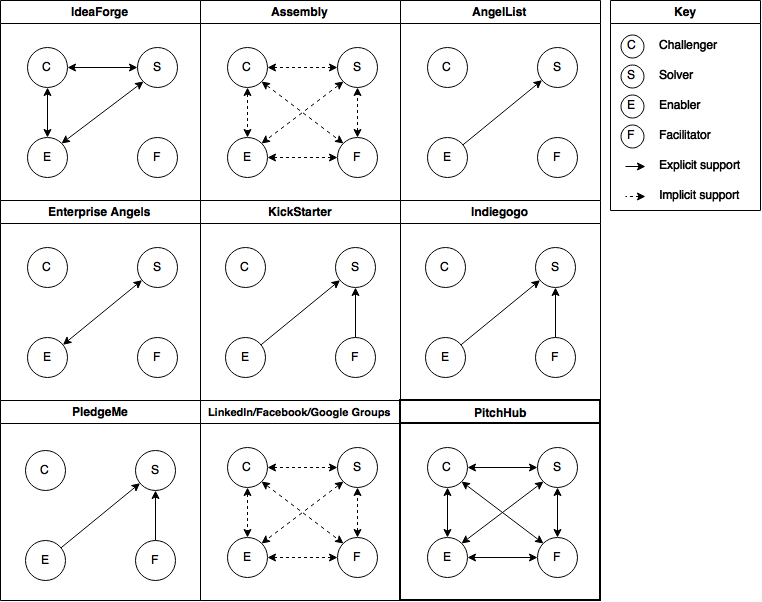
\includegraphics[width=1\textwidth]{collaborative_platforms}
    \caption{All collaborative platforms investigated do not provide explicit collaboration support between the all roles identified in Section \ref{commonRolesInInnovation}. PitchHub aims to fix this by supporting networking between all roles. }
    \label{fig:collaborative_platforms}
\end{figure}

As demonstrated in Figure \ref{fig:collaborative_platforms} PitchHub seeks to fill the gap in the online innovation collaboration space by being a platform that supports explicit collaboration between all roles. Throught this PitchHub aims to systematically build valuable business connections centered around the ideas. PitchHub has also been designed to incorporate features from the investigated platforms. From FaceBook, PitchHub extends its privacy control model with scope of disclosure negotiation, this is discussed later in Section TODO.

\section{Database Security}
Securely storing data is a large and increasingly important research area to modern society. In recent years companies like Sony, Apple and Adobe have experienced data breaches resulting in compromised user data. In a system like PitchHub where commercially sensitive information is being handled extreme care must be taken to ensure its safety.

\subsection{Threshold Security Schemes}
Secret Sharing schemes are a type of Threshold Security Scheme where a piece of data is split into \textit{n} secret shares. To retrieve the original data a threshold of \textit{k} of \textit{n} shares ("\textit{k}, \textit{n}") must be met before the original piece of data can be decrypted. A fictional scenario that describes this concept is where the code for launching a nuclear missile is split between three officers, to launch the missile all three officers must be present to reconstruct the launch code. Each share in isolation cannot be used to launch the missile, nor can it be used to infer the original code. This "3, 3" example is somewhat contrived but it showcases the fundamentals of secret sharing in that: the secret can be recovered given the threshold is met and the secret is indeed secret when any combination of \textit{t} shares are less than \textit{k}.

\subsection{Shamir's Secret Sharing Scheme}
Shamir's secret sharing \cite{shamir1979share} is a threshold scheme based on polynomial interpolation. 

\[q(x) = a_o +a_1x + ... + a_{k-1}x^{k-1} \]

The fundamental idea is that given a "\textit{k}, \textit{n}" scheme a random polynomial of degree \textit{k}-1 may be generated where the secret \textit{D} is hidden as term \(a_o\). A set of \textit{n} points may then be constructed from this polynomial and shared to \textit{n} secret keepers. To recover the secret \textit{D} the process requires a subset of \textit{k} secret shares to calculate the coefficients of the polynomial using interpolation. With this a system is able to recover the secret \textit{D} at term \(a_o\).
\par
Shamir's Secret Sharing scheme effectively allows a system to share secrets to \textit{n} secret keepers while maintaining each secret's safety as a long as a threshold of \textit{k} malicious secret keepers is not met. Besides being secure, Shamir's Secret Sharing scheme holds a number of other useful properties such as being minimal, extensible and dynamic \cite{shamir1979share}. The scheme is minimal in that the the size of each share does not exceed the size of the original secret. The scheme is extensible in that \textit{n} may be increased by giving new secret keepers new points from the polynomial. The scheme is dynamic in that the shares may be changed by modifying the polynomial but retaining the term \(a_o\).
\par
As discussed in a number studies the simplicity of Shamir's Secret Sharing scheme does present limitations that have the potential for being exploited \cite{abdallah2015analysis}\cite{dautrich2012security}. First, complete trust is given to the system who is dealing the secret shares, if an error occurs the secret may be irrecoverable therefore the system dealing the shares can be seen as a single point of failure. Second, Shamir's Secret Sharing scheme cannot detect secret keepers that cheat by supplying wrong shares, this brings about the problem where if \textit{k} members are compromised not only will the secrets be recoverable by the malicious party but the compromised members may be used to supply wrong secret shares to the system, effectively denying the first party system of recovering secrets. To combat these exploits Shamir's Secret Sharing may be extended with signature schemes \cite{shoup2000practical}\cite{abdalla2001forward} and verification schemes that do not assume the party dealing the shares is honest or infallible \cite{herzberg1995proactive}\cite{cachin2002asynchronous}.
